% Standalone TikZ sequence diagram: Client-Server communication (Agent 4).
% Compile with: pdflatex Seq_Agent4_ClientServer.tex
% Export to PNG if needed for inclusion in other tools.
\documentclass[tikz,border=2mm]{standalone}
\usepackage{tikz}
\usetikzlibrary{arrows.meta}
\begin{document}
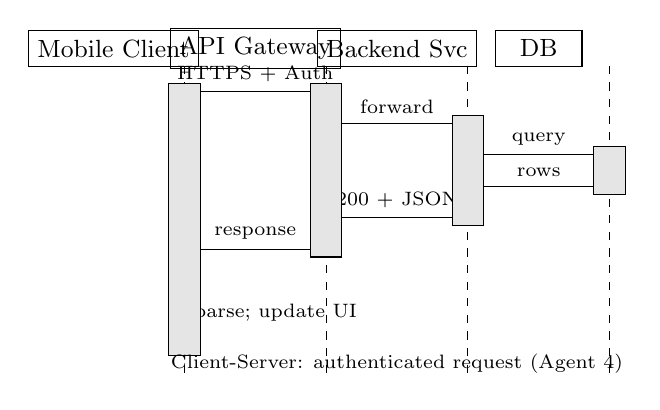
\begin{tikzpicture}[
    every node/.style={font=\small},
    participant/.style={rectangle, draw, minimum width=1.1cm, minimum height=0.45cm},
    arrow/.style={->, >=stealth}
]
    \node[participant] (client) at (0,0) {Mobile Client};
    \node[participant] (gw) at (1.8,0) {API Gateway};
    \node[participant] (svc) at (3.6,0) {Backend Svc};
    \node[participant] (db) at (5.4,0) {DB};

    \draw[dashed] (0.9, -0.22) -- (0.9, -4.2);
    \draw[dashed] (2.7, -0.22) -- (2.7, -4.2);
    \draw[dashed] (4.5, -0.22) -- (4.5, -4.2);
    \draw[dashed] (6.3, -0.22) -- (6.3, -4.2);

    \draw[arrow] (0.9, -0.55) -- (2.7, -0.55) node[midway, above, font=\scriptsize] {HTTPS + Auth};
    \draw[arrow] (2.7, -0.95) -- (4.5, -0.95) node[midway, above, font=\scriptsize] {forward};
    \draw[arrow] (4.5, -1.35) -- (6.3, -1.35) node[midway, above, font=\scriptsize] {query};
    \draw[arrow] (6.3, -1.75) -- (4.5, -1.75) node[midway, above, font=\scriptsize] {rows};
    \draw[arrow] (4.5, -2.15) -- (2.7, -2.15) node[midway, above, font=\scriptsize] {200 + JSON};
    \draw[arrow] (2.7, -2.55) -- (0.9, -2.55) node[midway, above, font=\scriptsize] {response};
    \draw[arrow] (0.9, -2.95) -- (0.9, -3.35) node[right, font=\scriptsize] {parse; update UI};

    \draw[fill=black!10] (0.7, -0.45) rectangle (1.1, -3.9);
    \draw[fill=black!10] (2.5, -0.45) rectangle (2.9, -2.65);
    \draw[fill=black!10] (4.3, -0.85) rectangle (4.7, -2.25);
    \draw[fill=black!10] (6.1, -1.25) rectangle (6.5, -1.85);

    \node[font=\scriptsize] at (3.6, -4.0) {Client-Server: authenticated request (Agent 4)};
\end{tikzpicture}
\end{document}
